\section{Overview}\seclabel{Overview}

\begin{figure}
\centering
\begin{tabular}{ccc}
\begin{lstlisting}
int sign(int x) { 
  int sgn;
  if (x < 0)
    sgn = -1
  else 
    sgn = 1
 return sgn
}
(*@ \vspace{0.1in} @*)
\end{lstlisting}
&
&
\begin{lstlisting}
int sign'(int x) {
  int sgn;
  if (x < 0)
    sgn = -1
  else if (x==0)
    sgn = 0
  else 
    sgn = 1
 return sgn
}
\end{lstlisting}
\\
\end{tabular}
\caption{Two simple implementations of the \emph{sign} operation.}
\figlabel{SignExample}
\end{figure}


Consider the simple example program of~\figref{SignExample}, inspired by an example from~\cite{MauborgneRival07}. For this example, we would like to establish that the output of $sign$ and $sign'$ only differ in the case where $x=0$ and that the difference is $sgn = 1 \neq sgn' = 0$. An optimal characterization of behavior is as following:
\\
\begin{tabular}{l|l|l}
$x.x'$ constraints  & $sgn$             & $sgn'$
\\ \hline
$x < 0$             & $sgn \mapsto -1$  & $sgn' \mapsto -1$
\\ \hline
$x = 0$             & $sgn \mapsto 1$  & $sgn' \mapsto 0$
\\ \hline
$x > 0$             & $sgn \mapsto 1$  & $sgn' \mapsto 1$
\end{tabular}
\\

As a first naive attempt to achieve such a description, one could try to analyze each version of the program separately and compare the (abstract) results. However, this is clearly unsound, as equivalence under abstraction does not entail concrete equivalence. For example, using a interval analysis~\cite{CousotHalbwachs78} would yield that in both programs the value of \scode{sgn} ranges in the same interval $[-1,1]$, missing the fact that $sign$ never returns the value $0$.

%\begin{wrapfigure}{r}{0cm}
%\imagetop{
%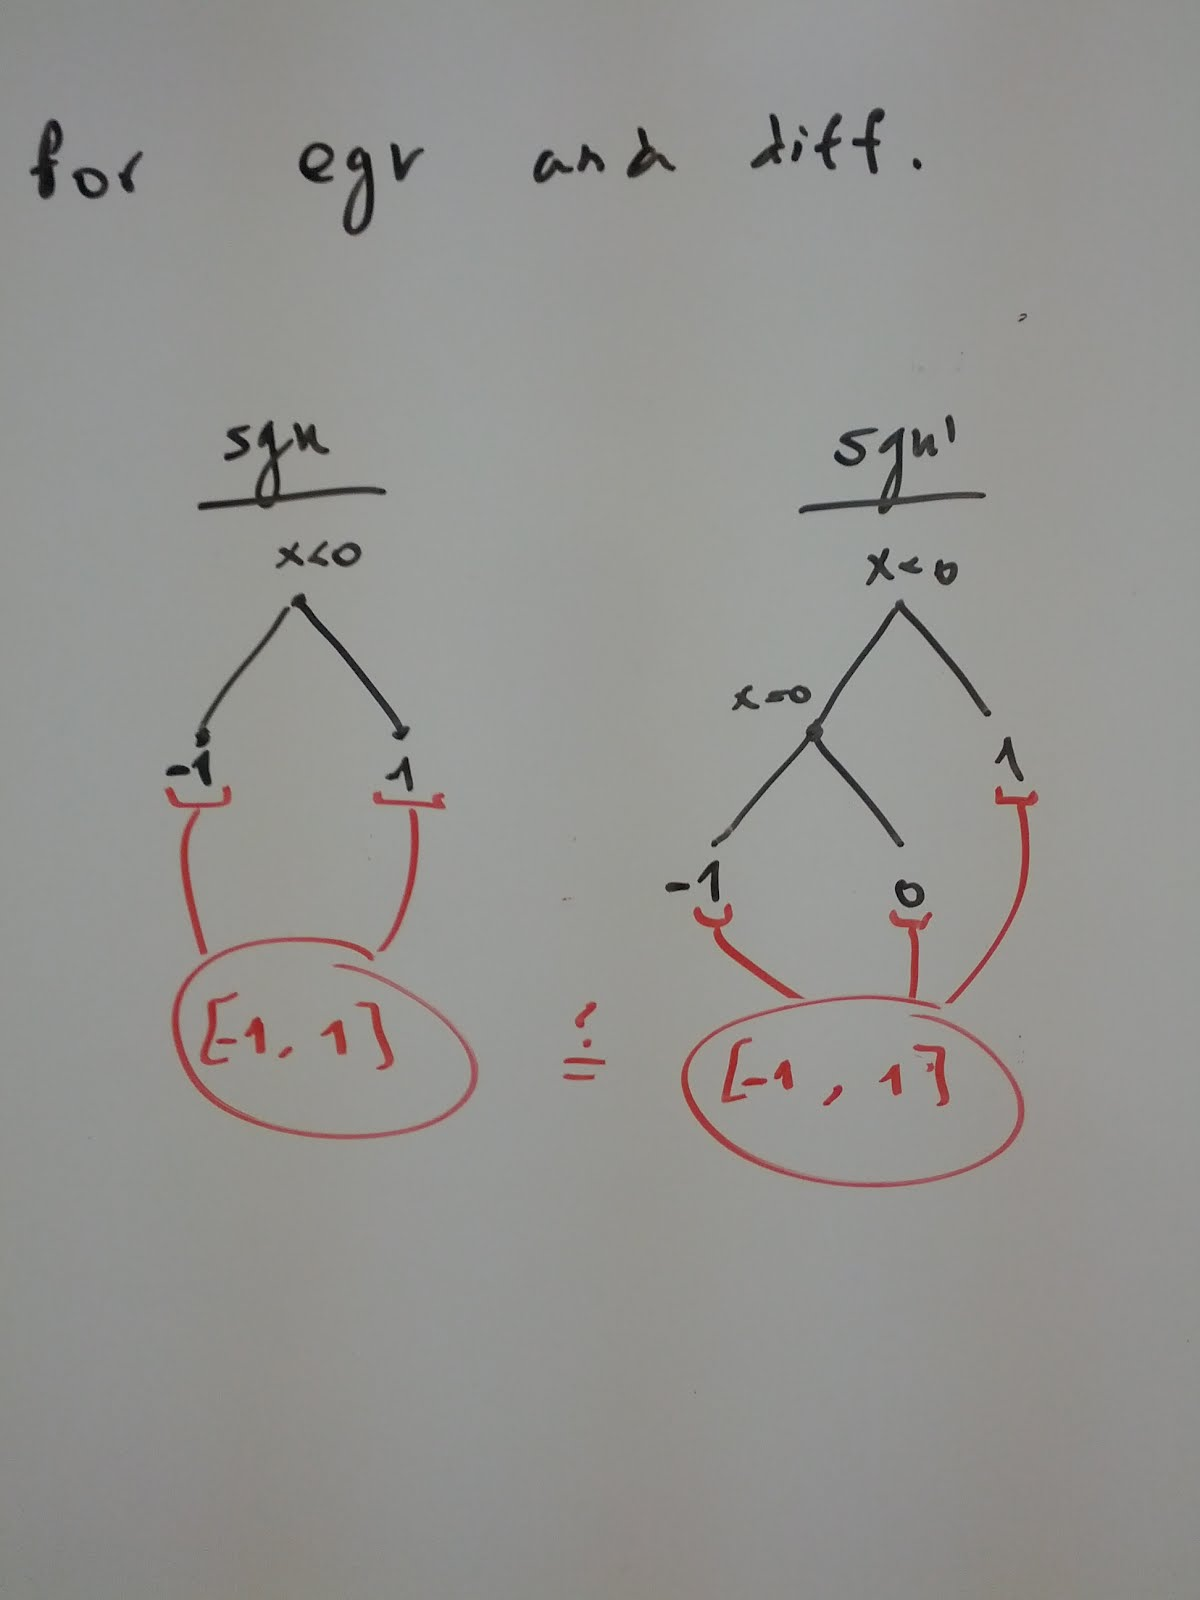
\includegraphics[scale=0.15,clip=true,trim = 125pt 400pt 125pt 350pt]{figures/sign-interval.jpg}
%}
%\caption{Interval analysis unsound comparison for $sign$ and $sign'$}\figlabel{SignInterval}
%\end{wrapfigure}

Furthermore, this result entirely ignores how $x$ affects the value of $sgn$ thus we would have no means to differentiate correctly, by input (e.g. we will get the same result for the $-1 * sign$ function).

To establish equivalence under abstraction, we need to abstract relationships between the values of variables in $sign$ and $sign'$ under the assumption of equivalence of input. Specifically, we need to track the relationship between the values of \scode{sgn} in both versions and see whether we can establish their equivalence. Tracking relationships dictates performing a \emph{joint analysis} that employs a \emph{correlating abstraction} allowing us to bind variables of both programs in one abstract state.

A correlating-oriented abstraction is well suited for proving equivalence as it allows focusing on relationships between versions of variables while abstracting away other (numerical) information allowing us to scale better. Most importantly, such an abstraction guarantees that equivalence will be reported soundly: as in a separate analysis we abstracted $\langle sgn \mapsto -1 \rangle$ and $\langle sgn \mapsto 1 \rangle$ towards an interval $\langle sgn \mapsto [-1,1] \rangle$, and again for $sgn'$ values, separately, which cannot assure equivalence (and in fact shouldn't). We instead use correlating states: $s_1 = \langle sgn = sgn' \mapsto -1 \rangle$ and $s_2 = \langle sgn = sgn' \mapsto 1 \rangle$, which allow us to abstract as such $s_1 \sqcup s_2 = \langle sgn = sgn', sgn \mapsto [-1,1] \rangle$ so equivalence can be soundly assured.

%If we instead use disjunctive completion powerset domain~\cite{TODO} where the abstract state is a set of convex sub-states, and no merge is ever performed, this would yield a precise result that may be used for equivalence checking and differencing.  For instance, using such domain for $sign$ would yield: $\langle x < 0, sgn = -1 \rangle \vee \langle x \geq 0, sgn = 1 \rangle$ and for $sign'$: $\langle x < 0, sgn = -1 \rangle \vee \langle x > 0, sgn = 1 \rangle \vee \langle x = 0, sgn = 0 \rangle$. Further refining $sign$'s abstraction and splitting the $\langle x \geq 0, sgn = 1 \rangle$ constraint to $\langle x > 0, sgn = 1 \rangle \vee \langle x = 0, sgn = 0 \rangle$ would allow perfectly aligning the input constraints to produce the difference of $x=0,sgn=1,sgn'=0$ as depicted in \figref{SignComplete}.
%\begin{wrapfigure}{r}{0cm}
%\imagetop{
%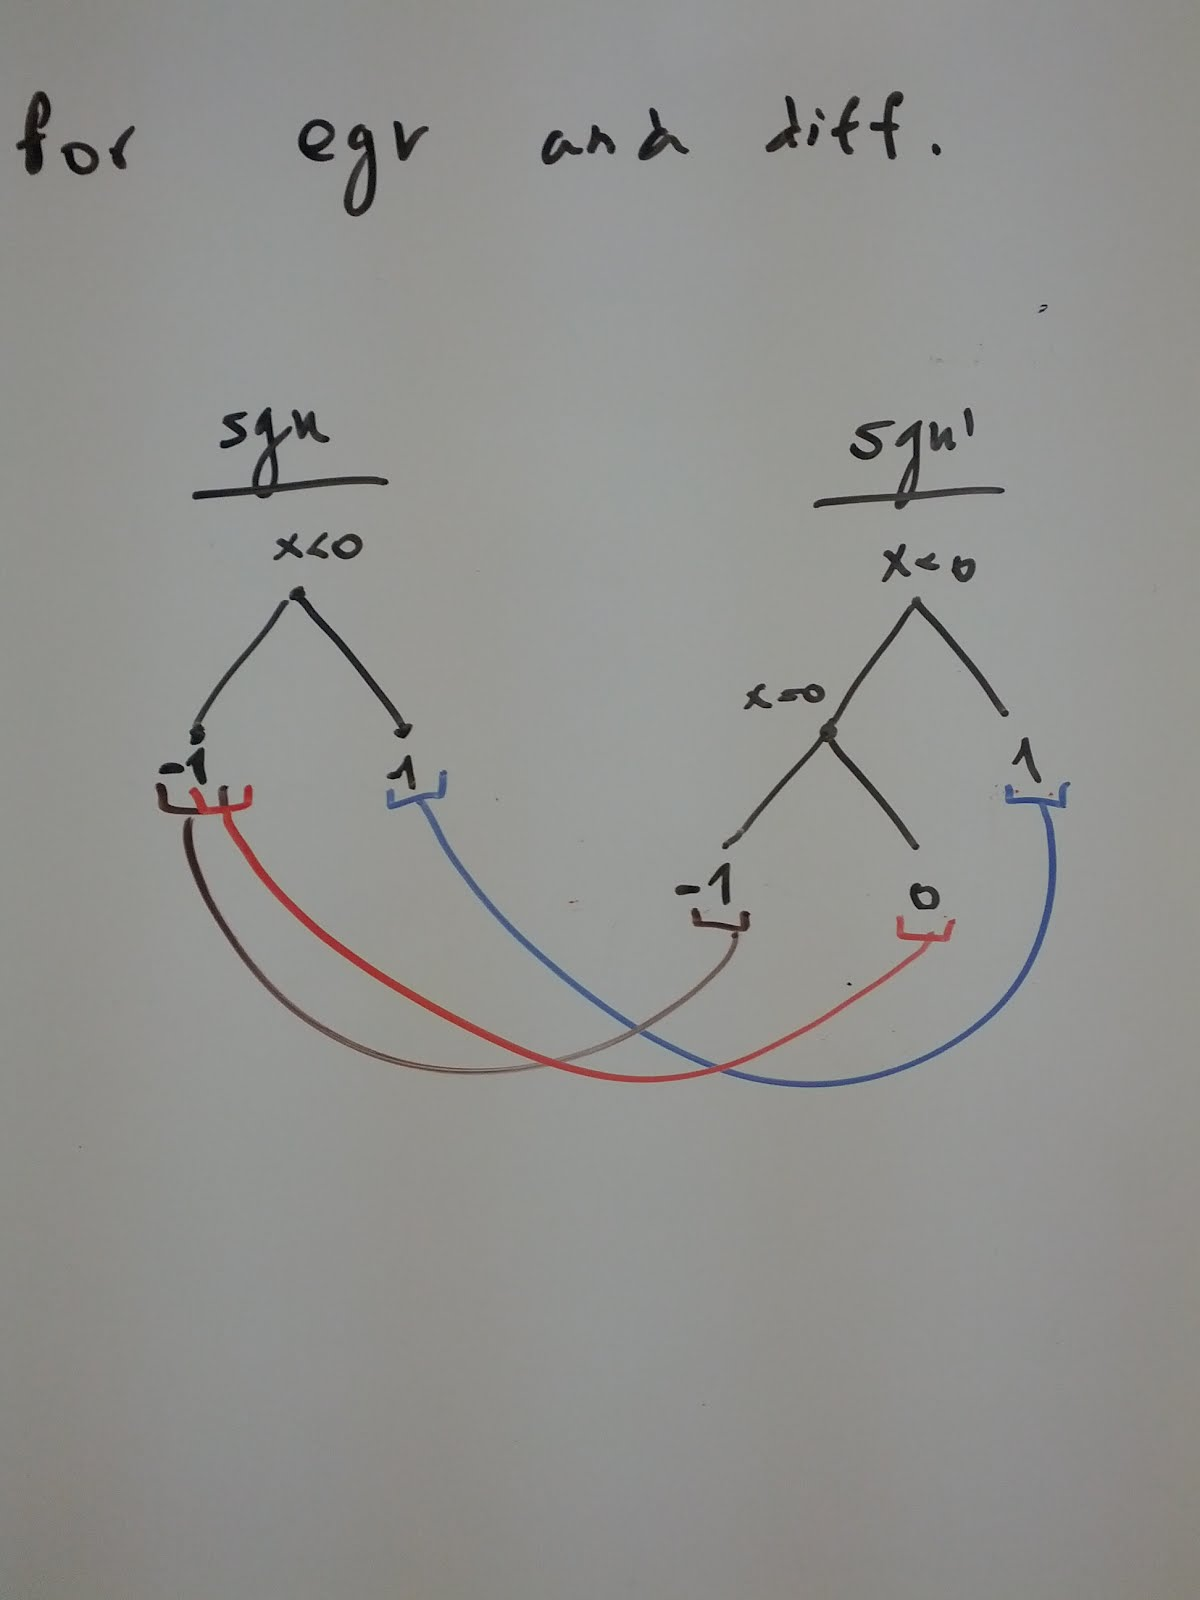
\includegraphics[scale=0.15,clip=true,trim = 125pt 450pt 100pt 350pt]{figures/sign-complete.jpg}
%}
%\caption{Complete disjunction analysis sound comparison for $sign$ and $sign'$}\figlabel{SignComplete}
%\end{wrapfigure}

We present an abstraction over dual program state, thats able to correlate paths that originate from the same input as well as produce a characterization of equivalence and difference which reflects change in behavior precisely. For example, we produce the following constraints for $sign$ and $sign'$:
\\
\begin{tabular}{ccc}
$\sigma_{\times}^1 = \{x = x' < 0, sgn = sgn' \mapsto -1\}$
\\
$\sigma_{\times}^2 = \{x = x' = 0, sgn \mapsto 1, sgn' \mapsto -1\}$
\\
$\sigma_{\times}^3 = \{x = x' > 0, sgn = sgn' \mapsto 1\}$
\\
\end{tabular}
\\

To arrive at this result, we used an initial setting which abstracted the dual program state by analyzing both programs sequentially ($P;P'$), while updating the shared state with data regarding both sets of variables, while allowing a complete disjunction over all paths. In order to correlate paths by input and arrive at a precise disjunction, the analysis initially assumes input equivalence $\vec{i} = \vec{i'}$.

In this setting, as we advance through the analysis of $P$, we will accumulate the disjunction of all possible path constraints in its final state (this is similar to trace partitioning~\cite{MauborgneRival07}). At this point, as we continue to analyze $P'$, each disjunct representing a path in $P$ will be further conjuncted with all of $P'$ paths. This will produce a precise disjunction for differencing as each path in $P$ will be split and conjuncted with all of $P'$ paths, while avoiding considering conjunctions that disagree on input due to our input equivalence assumption. An illustration of the joint analysis for the $sign$ example can be seen in \figref{SignAnalysis1} including markings for feasible and infeasible paths.

%In some cases, it would have been sufficient to use alternative domains that are capable of representing richer information, such as interval polyhedra~\cite{CMWC:SAS09}, or other numerical domains that can represent non-convex information (e.g., \cite{TODO}). The recent donut domain~\cite{GIBMG:VMCAI12} may be of particular interest for this purpose. However, the general principle of having to preserve correlating information even when information about the values is abstracted away, holds in all of these cases.

%\begin{figure}
%\imagetop{
%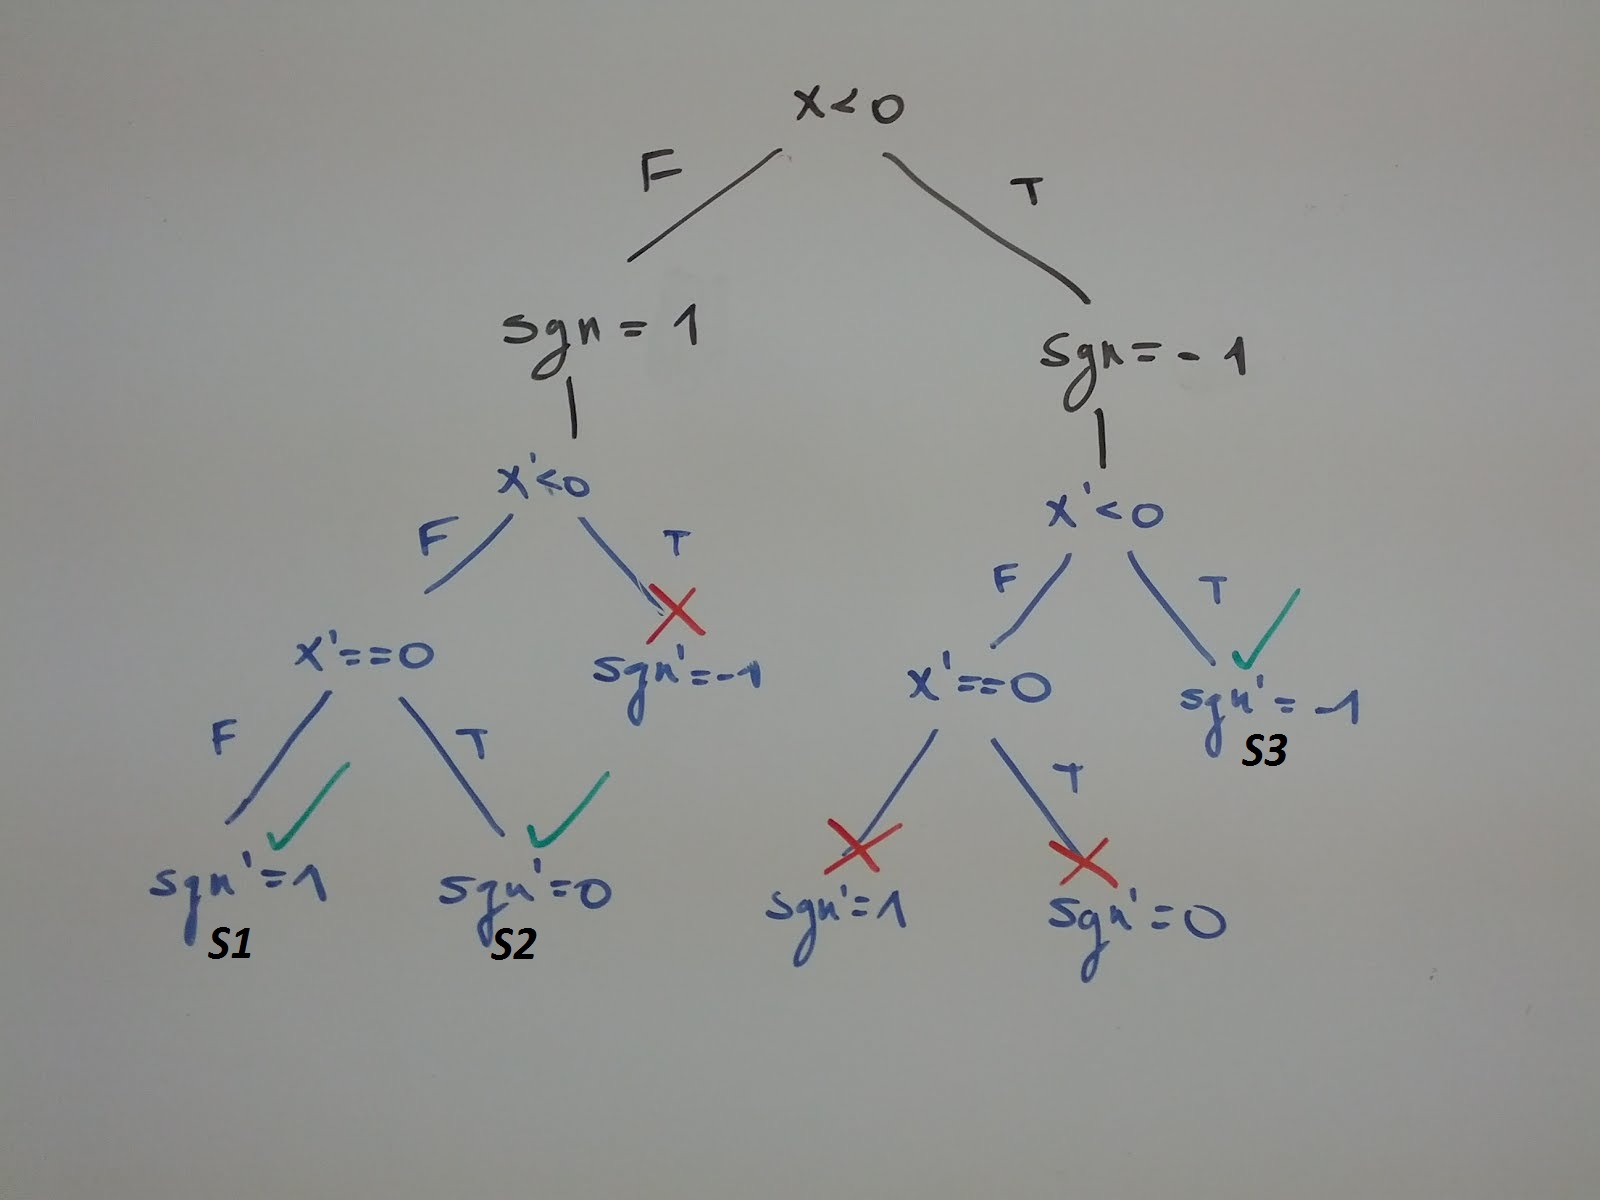
\includegraphics[scale=0.28,clip=true,trim = 50pt 100pt 100pt 0pt]{figures/sign-analysis1.jpg}
%}
%\caption{Joint $sign;sign'$ analysis}\figlabel{SignAnalysis1}
%\end{figure}

\begin{figure}
\centering
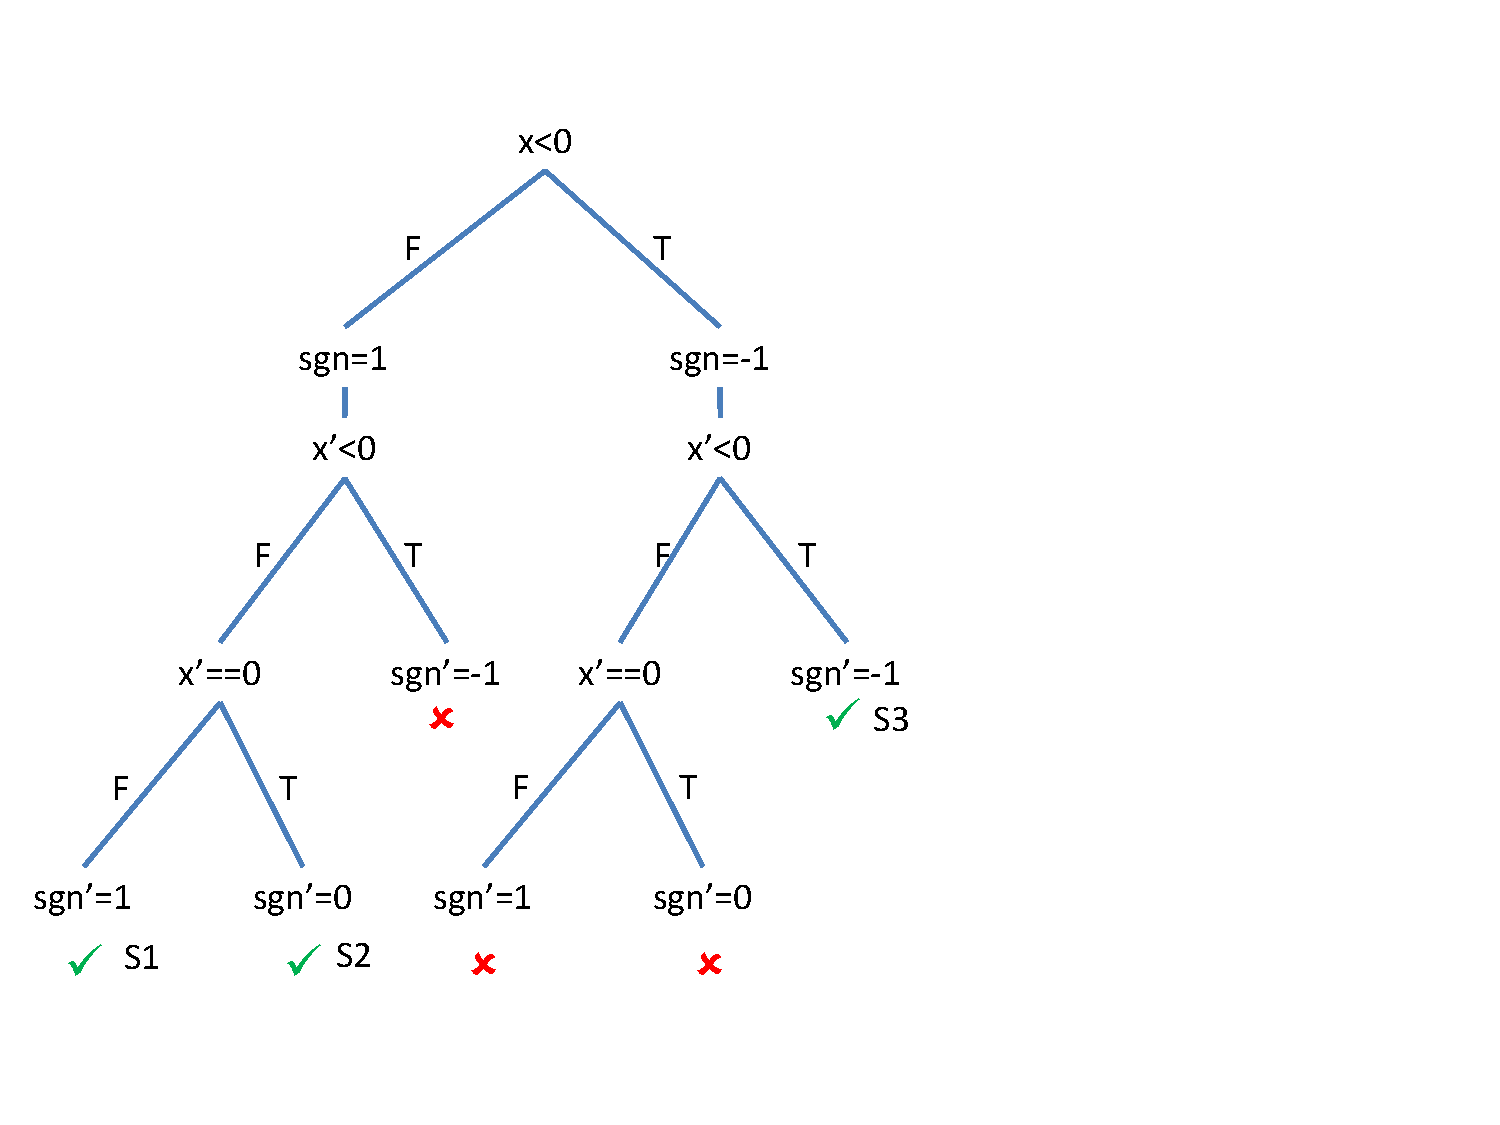
\includegraphics[scale=0.38,clip=true,trim = 75pt 25pt 5pt 20pt]{figures/sign-graph-joint}
\caption{Joint $sign;sign'$ analysis}\figlabel{SignAnalysis1}
\end{figure}

Essentially, our analysis aims to establish correspondence between paths in $P$ and $P'$ by first analyzing all of $P$ paths and then attempting to correlate with $P'$ paths. Clearly, this abstraction is unfeasible for most cases as the number of paths to be considered is exponential (we defer the case of loops where this number is unbound). Therefore we refine our abstraction by using a partially disjunctive domain, partitioned by \emph{equivalence criteria}.

%However, analyzing over $P;P'$ means in the worst case remembering the states along each $P$-path and relating them to states in the corresponding $P'$-path. This approach is similar to the symbolic execution approach~\cite{} where all possible correlating paths are explored individually and output is examined to determine difference whilst attempting to reach full coverage. Much like this approach, this abstraction is unfeasible for most cases, especially for programs with an unbound number of paths e.g. \textbf{loops}. To avoid this we move to a partially disjunctive domain, partitioned by \emph{equivalence criteria}.

As the goal of work is to distinguish equivalent from differencing behaviors, using equivalence as criteria for merging paths is apt. The partitioning will abstract together paths that hold equivalence for the same set of variables, allowing for a maximum of $2^{|VC|}$ disjunctions in the abstract state, where $VC$ is the set of correlated variables. So far we have implicitly defined $VC$ as a correlation between $P,P'$ input and outputs, but our approach is in fact parameterized by this matching, allowing for any $P$ variable to be matched with any of $P'$ which has the potential to provide a more precise result (in the cost of scaling) or alternatively provide a more coarse, scalable result by allowing less variables or only certain equivalence classes of $2^{VC}$. A formal definition and discussion of $VC$ is found in \secref{ConcreteSem}.

For example partitioning the result of \figref{SignAnalysis1} according to our criteria would abstract behaviors $s_1$ and $s_3$ together, as they hold equivalence for $sgn$. The merge would abstract away data regarding $x$ and represent $sgn$ as the $[-1,1]$ interval, losing precision but gaining reduction in state size. This lose of precision is acceptable as it is complemented by the offending state $s_2$. Still, not much is gained from this partitioning, as it is performed at the final state, where we may have already reached an exponential amount of disjunctions.

\begin{figure}
\centering
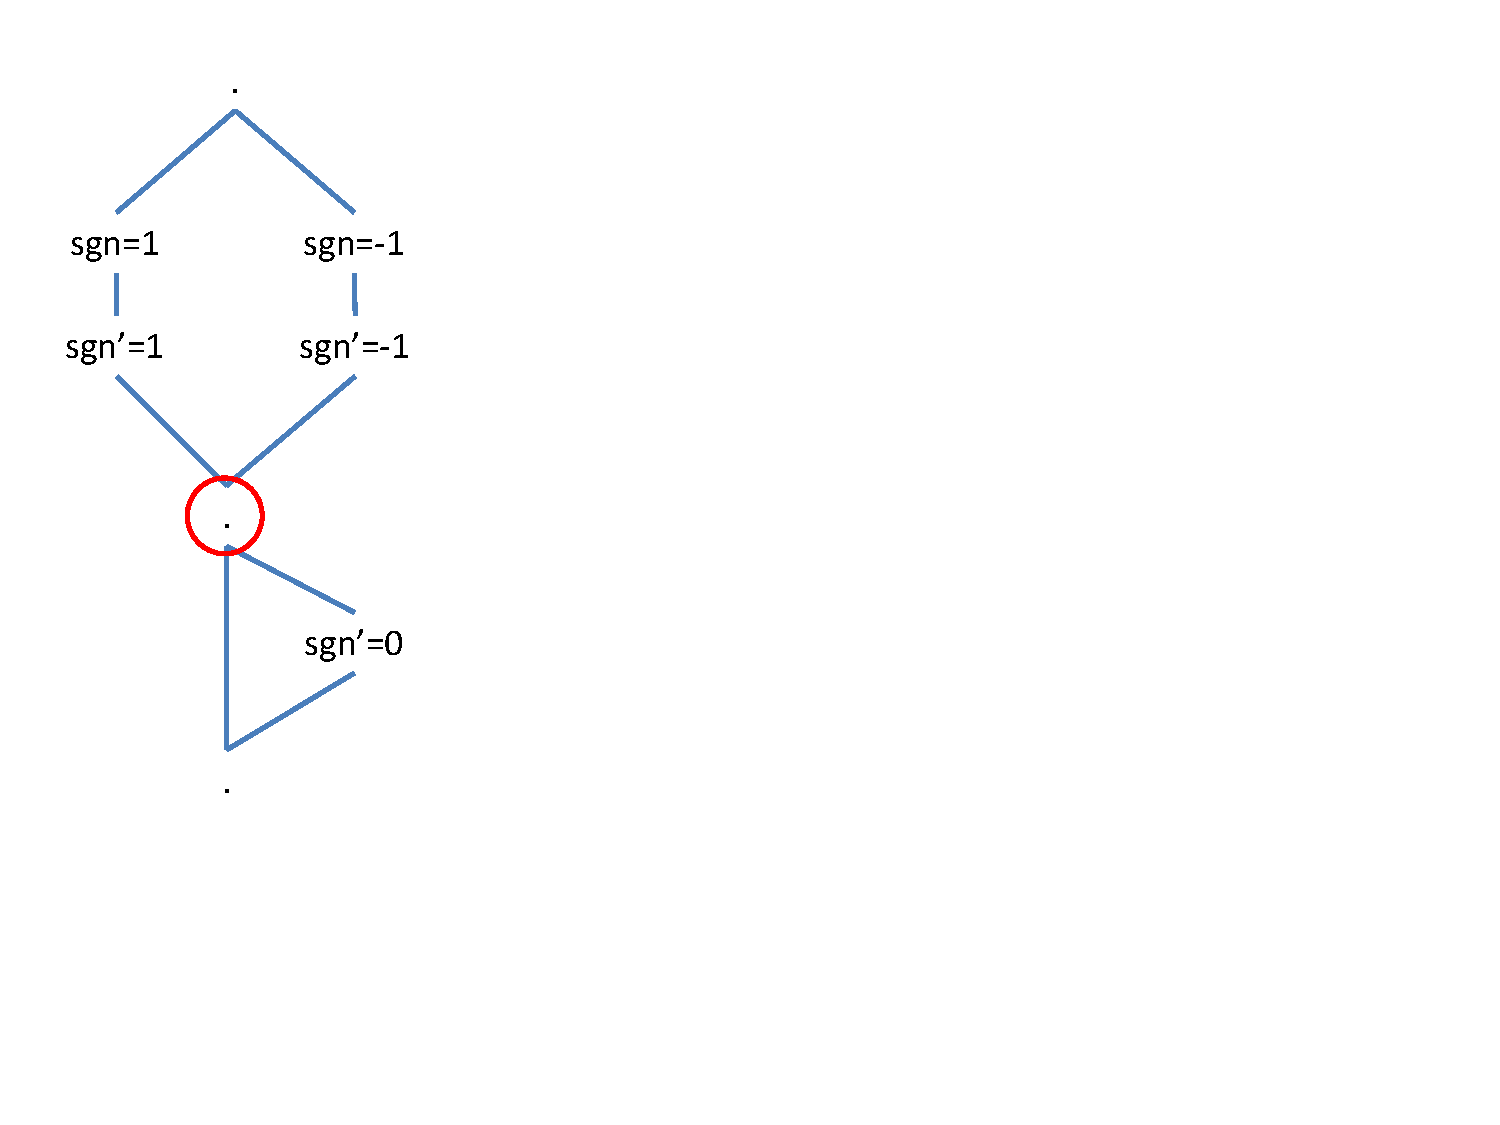
\includegraphics[scale=0.42,clip=true,trim = 0pt 150pt 450pt 150pt]{figures/sign-graph-correlated}
\caption{$sign \bowtie sign'$ analysis}\figlabel{SignAnalysis2}
\end{figure}

To truly gain a reduction of state size, we must perform partitioning dynamically as the analysis is executed i.e. at earlier program locations. This cannot be achieved using a sequential composition $P;P'$. Looking at \figref{SignAnalysis1} we immediately see that equivalence holds only at final states. Intuitively, this is caused due to a command in $P$ having to "wait" for its equivalent command to arrive in $P'$. To overcome this, we present the correlating program $P \bowtie P'$ which allows for earlier partitioning by "saving the need to wait". $P \bowtie P'$ interleaves $P$ and $P'$ commands in an optimized manner, and informs the analysis that it need not wait any further and partitioning is permitted. \figref{SignAnalysis2} depicts the analysis of $sign \bowtie sign'$ (shown in \figref{SignCorrelating}) where the partitioning location is marked with a circle. We define these partitioning locations as \emph{correlation points} (denoted $CP$) and they are a sub product of the correlating program build process. We will further describe the specifics of creating $P \bowtie P'$ in \secref{Correlating} and only shortly say that the interleaving is chosen according to a syntactic diff process over a guarded command language version of the programs.

\begin{figure}
\centering
\begin{lstlisting}
// Nimrod - please fill this 
\end{lstlisting}
\caption{Correlating program $sign \correlate sign'$.}
\figlabel{SignCorrelating}
\end{figure}


% bite the bullet and do widening.
Although we achieved a reduction in state size using partitioning, we have yet to account for programs with an unbound number of paths, created by loops. Unbound path lengths means a potentially unbound analysis as all paths are abstracted. This is mainly where previous approaches fall short ~\cite{GodlinStrichman09, KawaguchiLahiriRebelo10, DwyerElbaumPerson08, EnglerRamos11}. To overcome this, we define a widening operator for our domain, based on the convex sub-domain widening operator. The main challenge here, as our state is a set of convex objects, is finding an optimal pairwise matching between objects for a precise widened result. Optimally, we would like to pair objects that adhere to the same "looping path" meaning we would want to match a path $\pi_i$'s abstraction with a path $\pi_{i+1}$ that results from taking another step in the loop. This basically requires encoding path information along with the sub-state abstraction. This information is acquired by simply keeping guard values explicitly, as they appear in our correlating program, inside the state. As guard values (true or false) reflect branch outcomes, they can be used to match sub-states that advanced on the loop by matching their guard values (for easier matching and better precision we separate guards from other variables in our implementation).

\begin{figure}
\centering
\begin{lstlisting}
int sum(int arr[], unsigned len) {
  int result = 0;
  for (unsigned i = 0; i < len; i++)
    result += arr[i];
 return result;
}
\end{lstlisting}
\caption{A simple looping program for array summation.}
\figlabel{LoopExample}
\end{figure}

We note that the correlating program is cruicial to maintaining equivalence over loops. To demonstrate this we perform the simple exercise of checking equivalence of a small looping program with itself. Consider the array summation program in \figref{LoopExample}. Equivalence for these two small programs cannot be established soundly by approached based on under approximation. To emphasize the importance of the correlating program, we will first show the result of an analysis of $sum;sum'$ which will be:
\\
\begin{tabular}{c}
$\sigma_{\times}^1 = \{len = len' \leq 1, result = result' \mapsto 0\}$
\\
$\sigma_{\times}^2 = \{len = len' > 1\}$
\end{tabular}
\\
\begin{figure}
\centering
\begin{lstlisting}
int sum(int arr[], unsigned len) {
  unsigned len' = len;
  int arr'[] = arr;
  int result = 0;
  int result' = 0;
  {
    unsigned i = 0;
    unsinged i' = 0;
l:  guard g = (i < len);
l': guard g' = (i' < len');
    if (g) result += arr[i];
    if (g') result' += arr'[i'];
    if (g) i++;
    if (g') i'++;
    if (g) goto l;
    if (g') goto l';
  }
}
\end{lstlisting}
\caption{$sum \bowtie sum$}
\figlabel{LoopExample}
\end{figure} 
This lose of equivalence occurred due to the inability precisely track the relationship of $result$ and $result'$ over $sum;sum'$. As we widened the first loop to converge, all paths passing through that loop were merges together, losing the ability to be "matched" with the second loop waiting further down the road. Performing the same analysis on $sum \bowtie sum'$ instead (seen in \figref{LoopCorrelatingExample}), allows maintaining equivalence, as the loops are interleaved correctly to allow establishing $result = result'$ as a loop invariant, surviving the widening process to prove equivalence at the end as the result would be:
\\
\begin{tabular}{c}
$\sigma_{\times}^1 = \{result = result'\}$
\end{tabular}
\\
%The conceptual difference of these two analyses is depicted in \figref{SumWidening}.
%\begin{figure}
%\imagetop{
%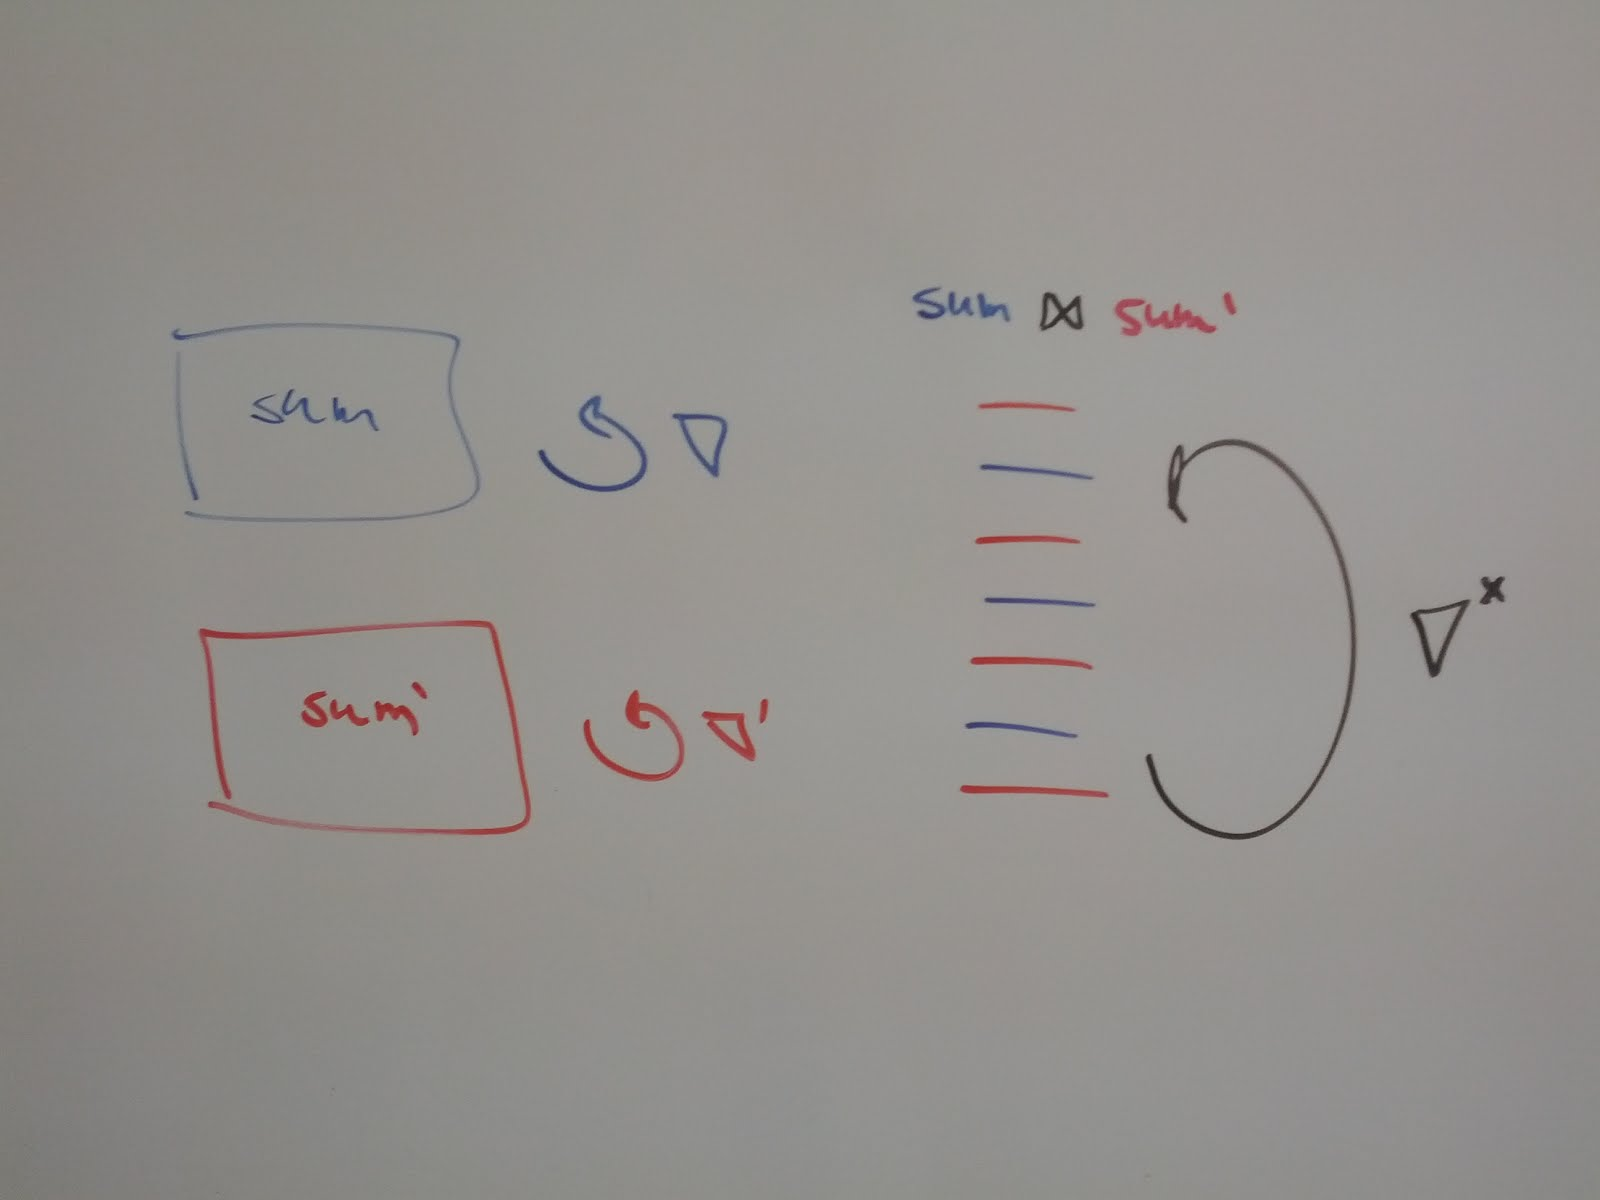
\includegraphics[scale=0.20,clip=true,trim = 150pt 250pt 200pt 200pt]{figures/sum-widening.jpg}
%}
%\caption{Widening $sum ; sum$ vs. $sum \bowtie sum$}\figlabel{SumWidening}
%\end{figure}

\paragraph{Definition of difference}
So far, we defined difference in programs as difference in output variable values at the program final state. Our work extends the notion of difference beyond that, allowing for several program locations to be identified as viable for differentiation (we name these locations \emph{differencing points} denoted $DP$). Other than the programs endpoints, we include every location which:
\begin{itemize}
\item Emits an output value (using a system function or through a global variable)
\item Accesses array
\end{itemize}
This means that procedures may now differ, even if they hold equivalence on the final state. Thus we define difference also as producing a different output value in mid-execution or accessing an array through a different index. This means that programs which differ in array access \emph{patterns} will now be flagged as different. This is a sound approach for difference, as this may include access to illegal bounds (an example for this can be seen in \figref{Md5sumExample}). We note that this definition of description cannot be achieved by instrumenting output or array access through temporary variables and deferring checking their equivalence to the end, as the amount of temporaries needed may be unbound. We therefore require procedures to agree on these locations, in case we wish to verify using the extended definition of difference.